\documentclass[a4paper,12pt]{article}
\usepackage{karnaugh-map}
\usepackage[utf8]{inputenc}
\usepackage{amssymb,amsmath}
\usepackage{float}

\usepackage[margin=1in]{geometry}
\usepackage{lipsum}
\usetikzlibrary{arrows, shapes.gates.logic.US, calc}
\tikzstyle{branch}=[fill, shape=circle, minimum size=3pt, inner sep=0pt]
    
\begin{document}
\newdimen\origiwspc%
\newdimen\origiwstr%


\section*{Task 3: Issues at minimal cost implementation}

Given a truth table, it was requested to see what happens
when the truth table is implemented with the smallest quantity of logic
gates. To perform this task, ICs that either have NOR 
or NAND logic gates will be used.

\subsection*{Low cost approach}
\begin{figure}[htbp]
    \begin{center}
    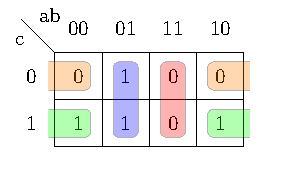
\includegraphics{karnaugh.pdf}
    
    \end{center}
    
    \caption{Karnaugh Map of the given truth table}
    \label{fig:KarnaughMap}
    \end{figure}
We can get the minimal cost output expressed either in groups of 
maxterms (orange and red groups) or minterms (blue and green groups).
\linebreak
Let Z be the output label, its reduced minterms expression is:
\begin{equation}
    Z= (\bar{A}.B)+(C.\bar{B})
\end{equation} 
Also, its reduced maxterms expression is:
\begin{equation}
    Z= (\bar{A}+\bar{B}).(C+B)
\end{equation} 
\begin{figure}[htbp]
    \begin{center}
        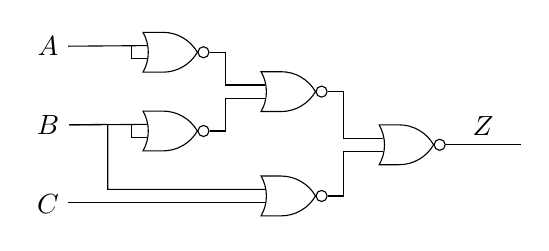
\begin{tikzpicture}
            %seteamos el orden de las variables
            \node (x) at (0, 2)(x) {$A$};
            \node (y) at (0, 1) (y){$B$};
            \node (z) at (0, 0)(z) {$C$};
        
            %creamos un nodo con una posicion asociada:($(x)) que es donde se encuentra
            %posicionada la variable x y le ponemos nombre: nor_x
            %los numeros son para desplazar la compuertas
            \node[nor gate US, draw, rotate=0, logic gate inputs=nn] at ($(x) + (1.5, -0.075)$) (nor_x) {};
            \node[nor gate US, draw, rotate=0, logic gate inputs=nn] at ($(y) + (1.5, -0.075)$) (nor_y) {};
            
            %dibujar la nor con las entradas unidas:
            %primero dibujamos una linea
            \draw (x) -- (nor_x.input 1); 
            % ahora dibujamos desplazada la linea que va a entrar al input 2
            \draw (nor_x.input 2) -- ([xshift=-0.2cm]nor_x.input 2) |- (nor_x.input 1);
        
            \draw (y) -- (nor_y.input 1);
            \draw (nor_y.input 2) -- ([xshift=-0.2cm]nor_y.input 2) |- (nor_y.input 1);
        
            %asigno dos entradas
            \node[nor gate US, draw, rotate=0, logic gate inputs=nn] at ($(x) + (3, -0.075-0.5)$) (norAndB) {};
            \draw (nor_x.output) -- ([xshift=0.2cm]nor_x.output) |- (norAndB.input 1);
            \draw (nor_y.output) -- ([xshift=0.2cm]nor_y.output) |- (norAndB.input 2);
        
            \node[nor gate US, draw, rotate=0, logic gate inputs=nn] at ($(z) + (3, 0+0.10)$) (norBandC) {};
            \draw (z) -- ([xshift=0.2cm]z) |- (norBandC.input 2);
            \draw (y) -- ([xshift=-0.5cm]nor_y.input 1)  |- (norBandC.input 1);
        
            \node[nor gate US, draw, rotate=0, logic gate inputs=nn] at ($(y) + (4.5, -0.25)$) (norFinal) {};
            \draw (norAndB.output) -- ([xshift=0.2cm]norAndB.output) |- (norFinal.input 1);
            \draw (norBandC.output) -- ([xshift=0.2cm]norBandC.output) |- (norFinal.input 2);
        
            \draw (norFinal.output) -- node[above]{$Z$} ($(norFinal) + (1.5, 0)$);
        \end{tikzpicture}
        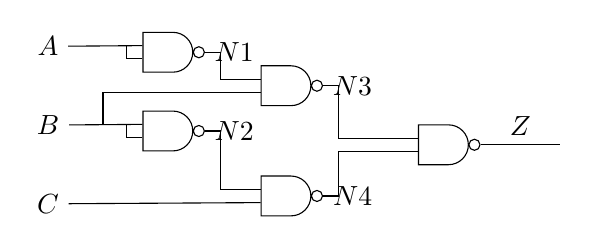
\begin{tikzpicture}
            \node (x) at (0, 2)(x) {$A$};
            \node (y) at (0, 1) (y){$B$};
            \node (z) at (0, 0)(z) {$C$};
            \node[nand gate US, draw, rotate=0, logic gate inputs=nn] at ($(x) + (1.5, -0.075)$) (nand_x) {};
            \draw (x) -- (nand_x.input 1); 
            \draw (nand_x.input 2) -- ([xshift=-0.2cm]nand_x.input 2) |- (nand_x.input 1);
            \draw (nand_x.output) -- node[right]{$N1$} ($(nand_x.output) + (0, 0)$);

            \node[nand gate US, draw, rotate=0, logic gate inputs=nn] at ($(x) + (3, -0.5)$) (nandAandB) {};
 


            \draw (nand_x.output) -- ([xshift=0.2cm]nand_x.output) |- (nandAandB.input 1) ;
            \node[nand gate US, draw, rotate=0, logic gate inputs=nn] at ($(y) + (1.5, -0.075)$) (nand_y) {};
            \draw (nand_y.output) -- node[right]{$N2$} ($(nand_y.output) + (0, 0)$);

            \draw (nandAandB.output) -- node[right]{$N3$} ($(nandAandB.output) + (0, 0)$);

            \draw (y) -- (nand_y.input 1); 
            \draw (nand_y.input 2) -- ([xshift=-0.2cm]nand_y.input 2) |- (nand_y.input 1);
            \draw (nand_y.input 1) -- ([yshift=0cm]nand_y.input 1) -- ([xshift=-0.5cm]nand_y.input 1) |- (nandAandB.input 2);
            \node[nand gate US, draw, rotate=0, logic gate inputs=nn] at ($(z) + (3,0.1)$) (nandBandC) {};
            
            \draw (nandBandC.output) -- node[right]{$N4$} ($(nandBandC) + (0.5, 0)$);
            
            \draw (z) -- (nandBandC.input 2); 
            \draw (nand_y.output) -- ([xshift=0.2cm]nand_y.output) |- (nandBandC.input 1);

            \node[nand gate US, draw, rotate=0, logic gate inputs=nn] at ($(y) + (5, -0.25)$) (nandFinal) {};
            \draw (nandAandB.output) -- ([xshift=0.2cm]nandAandB.output) |- (nandFinal.input 1);
            \draw (nandBandC.output) -- ([xshift=0.2cm]nandBandC.output) |- (nandFinal.input 2);
            \draw (nandFinal.output) -- node[above]{$Z$} ($(nandFinal) + (1.5, 0)$);

        \end{tikzpicture}



    \end{center}
    \caption{Implementation with NOR gates and NAND gates respectively}
\end{figure} 

Note that the quantity of logic gates in both cases are the same.

\section*{Glitch analysis}
Sometimes propagation delays cause unexpected and unwanted transition 
in the ouput. This issue is called 'glitch' and it's related to how 
the logical circuit is synthesized. In this section, the NAND implementation
 will be taken into account.
If we take into accout the propagation time of the NAND logic gate
(here we assume all propagation times are equal) and then observe transition
 of the states A,B,C from 011 to 001 respectively.


\begin{figure}[H] 
    \begin{center}
    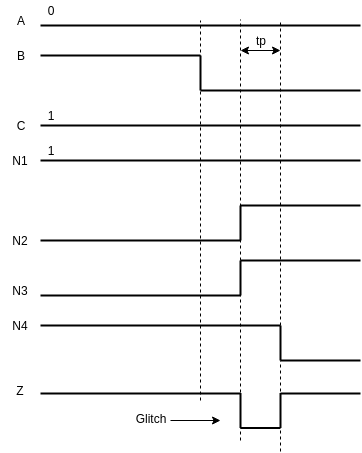
\includegraphics[width=7cm,height=9cm]{glitch.png}
    \end{center}
    \caption{Propagation time analysis}
    \label{fig:proptime}
    \end{figure} 
Note that the interval of time tp in Figure~\ref{fig:proptime}  denotes the propagation time.
\linebreak
The result might be at first surprising but  in fact this effect was in someway
expected. Take a look at the Karnaugh map in Figure~\ref{fig:KarnaughMap}.
An input that follows multiple paths to an output can create a glitch if 
one path has an inverter (in this case implemented with a NAND logic gate) 
and one does not. This issue is called "asymmetric path delay" and it can be
seen in Figure~\ref{fig:KarnaughMap} with the input B.

\section*{Conclusion}
In order to remove glitches it is needed to add redundant groups in the
Karnaugh Map so that disjoint groups overlap.
\begin{figure}[H] 
    \begin{center}
    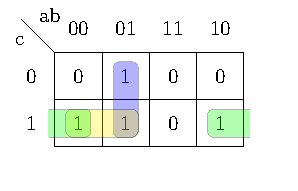
\includegraphics{karnaugh_improved.pdf}
    \end{center}
    \caption{Improved karnaugh}
    \label{fig:karnaugh_improved}
    \end{figure} 
In this case the output is given by:
\begin{equation*}
    Z= (\bar{A}+\bar{B}).(C+B)+(\bar{A}.C)    
\end{equation*} 

Note that the new term added to the expression is not dependent
of B so regardless of the variation of B there won't be glitches
in the output, because it will be fixed by this new term.
\linebreak
Finally to give some sense to the adding some redundant logic,
when we make Karnaugh groups we take the non-changing states and
the only variable that changes of state in the new group is B
which is reasonable due to the fact that that's the variable 
causing the issue.
Depending on the application it may be important or not to remove
glitches.
There might be more glitches, remember that this is just one particular case,
where glitches are more likely to happen.
\end{document}